\documentclass[11pt]{article}
\usepackage[margin=0.75in]{geometry}
\usepackage{amsmath}
\usepackage{tikz}
\usepackage{enumitem}
\usepackage{siunitx}
\setlength{\parindent}{0pt}
\newcommand{\graphbox}{\begin{center}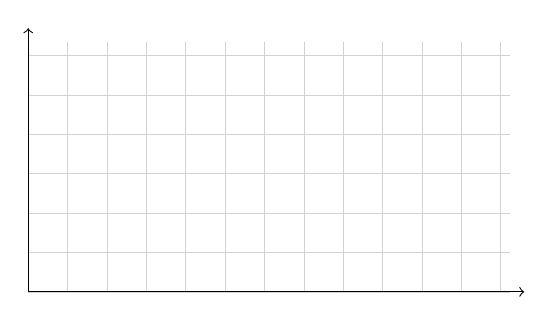
\begin{tikzpicture}[x=0.72cm,y=0.72cm]
\draw[step=0.5cm,gray!35,very thin] (0,0) grid (8.5,4.4);
\draw[->] (0,0)--(8.75,0); \draw[->] (0,0)--(0,4.65);
\end{tikzpicture}\end{center}}
\begin{document}
\begin{center}\Large\textbf{AP Physics 1 1D Motion Post-Lab Quiz -- Version C}\end{center}
\vspace{0.08in}\textbf{Name:} \rule{2.1in}{0.4pt}\hfill\textbf{Period:} \rule{0.65in}{0.4pt}\hfill\textbf{Date:} \rule{1.1in}{0.4pt}
\vspace{0.12in}
\begin{enumerate}[leftmargin=*,itemsep=0.15in]
\item A student repeatedly releases the same ball from the same marked height and measures its motion while it falls.

\textbf{a.} Describe how the repeated trials should be performed so that they can be fairly compared.\\
\textbf{b.} Explain one reason repeated trials can improve the quality of the experimental results.
\vspace{0.55in}

\item A student originally uses a handheld stopwatch while observing a ball fall from a fixed height. The student decides instead to record the fall with a phone.

\textbf{a.} Explain how the student could use the video to measure time during the fall.\\
\textbf{b.} Explain why using recorded video could give more precise measurements than manually operating a stopwatch.
\vspace{0.55in}

\item A student records the motion of a ball released from rest during free fall.

\begin{center}
\begin{tabular}{c|cccccc}
Time $t$ (s) & 0.00 & 0.10 & 0.20 & 0.30 & 0.40 & 0.50\\ \hline
Distance fallen $d$ (m) & 0.000 & 0.049 & 0.198 & 0.439 & 0.787 & 1.224
\end{tabular}
\end{center}
\textbf{a.} Transform the data as needed to produce a linear graph. Using the graph space provided, plot the appropriate variables, clearly label both axes with units, and draw a best-fit line.\\
\textbf{b.} Describe the shape of your graph. Based on the graph, determine whether the ball's acceleration was approximately constant and explain your reasoning.

\graphbox
\end{enumerate}
\end{document}
